% Template for NIME 2015
%
% Modified by Edgar Berdahl on 5 November 2014
% Modified by Baptiste Caramiaux on 25 November 2013
% Modified by Kyogu Lee on 7 October 2012
% Modified by Georg Essl on 7 November 2011
%
% Based on "sig-alternate.tex" V1.9 April 2009
% This file should be compiled with "nime2011.cls"
%

\documentclass{nime-alternate}

\begin{document}
%
% --- Author Metadata here ---
%\conferenceinfo{NIME'16,}{July 11-15, 2016, Griffith University, Brisbane, Australia.}

\title{Granabular: a collaborative granular synthesizer}

%
% You need the command \numberofauthors to handle the 'placement
% and alignment' of the authors beneath the title.
%
% For aesthetic reasons, we recommend 'three authors at a time'
% i.e. three 'name/affiliation blocks' be placed beneath the title.
%
% NOTE: You are NOT restricted in how many 'rows' of
% "name/affiliations" may appear. We just ask that you restrict
% the number of 'columns' to three.
%
% Because of the available 'opening page real-estate'
% we ask you to refrain from putting more than six authors
% (two rows with three columns) beneath the article title.
% More than six makes the first-page appear very cluttered indeed.
%
% Use the \alignauthor commands to handle the names
% and affiliations for an 'aesthetic maximum' of six authors.
% Add names, affiliations, addresses for
% the seventh etc. author(s) as the argument for the
% \additionalauthors command.
% These 'additional authors' will be output/set for you
% without further effort on your part as the last section in
% the body of your article BEFORE References or any Appendices.

\numberofauthors{1} %  in this sample file, there are a *total*
% of EIGHT authors. SIX appear on the 'first-page' (for formatting
% reasons) and the remaining two appear in the \additionalauthors section.
%
\author{
% You can go ahead and credit any number of authors here,
% e.g. one 'row of three' or two rows (consisting of one row of three
% and a second row of one, two or three).
%
% The command \alignauthor (no curly braces needed) should
% precede each author name, affiliation/snail-mail address and
% e-mail address. Additionally, tag each line of
% affiliation/address with \affaddr, and tag the
% e-mail address with \email.
%
% 1st. author
\alignauthor
Christian Steinmetz\\
       \affaddr{Universtat Pompeu Fabra, Barcelona}\\
       \email{christianjames.steinmetz01@estudiant.upf.edu}
}

\maketitle

\begin{abstract}

Granabular is a networked, multi-user granular synthesizer with a lightweight web-based interface. 
The aim of this work is to provide a means to generate collaborative soundscapes, 
in real-time using a single granular engine implemented in Pure Data. A web-server, 
built in Flask, manages communication between the users, who connect via any web browser, and the granular engine. 
Users are randomly assigned a different parameter of the synthesizer to control, 
and also have the ability to enter search queries, which are used to download recordings 
from Freesound to be used as source files in the synthesizer. 
In addition, users will be periodically prompted to generate sounds that will be recorded 
by their device and sent to the server to be used as source files. Granabular is designed with a minimalist 
interface so as to provide a low barrier of entry for participants and aims to enable a paradigm of 
collaboration between users interacting with a single instrument. 

\end{abstract}

\keywords{NIME, proceedings, \LaTeX, template}

\section{Introduction}
In 1947, Garbor proposed his concept of acoustical quanta, wherein any sound could be described from a quantum perspective, 
which ultimately laid the foundation for the development of granular synthesis \cite{gabor1947acoustical}. 
The concept of granular synthesis was first formalized from a compositional standpoint by Iannis Xenakis in the early 1970s, 
wherein he described the process of describing any given sound by a set of fundamental sound units known as grains \cite{xenakis1992formalized}. 
These sonic grains are small sound events generally 1 - 50 ms that are played back in rapid succession to generate a more significant acoustic event \cite{roads1988granular}. 
Xenakis experimented with this concept in practice through the use of precise tape-splicing, 
but such methods proved challenging given their technological limitations \cite{roads1996computer}. 
As digital audio technologies evolved granular synthesis techniques became more accessible and composers 
such as Barry Truax \cite{truax1988real} and Curtis Roads \cite{roads1988granular} became heavily involved 
in the development of digital systems for granular synthesis. As the technology has evolved, 
many commercial devices have been developed that provide composers and musicians with the ability to perform granular synthesis with ease. 

Granabular aims to extend upon these past implementations of granular synthesis, not with the introduction of new synthesis techniques, 
but with a new method of human-computer interaction in the compositional process through a collaborative system. 
While previous collaborative synthesis systems have been proposed, the contributions of this work are two-fold:

\begin{enumerate}
	\item A minimalist user interface that requires no knowledge of synthesis techniques.
	\item Sourcing of grains from user devices and user driven creative commons libraries. 
\end{enumerate}

By enabling multiple users to connect to the same granular engine simultaneously, 
each with control over a unique parameter, no single user is in complete control of the synthesis process, 
leading to potentially interesting and unpredictable outcomes. 

\section{Related work}

Collaboration is a foundational aspect of many forms of music creation from the choir to the orchestra, 
to the contemporary four-piece rock band. 
Although, notably this collaboration nearly always occurs among skilled performers each playing their own instrument. 
Some early exceptions include four handed piano compositions, 
wherein two performers play the same piano concurrently \cite{kuhn2001music}, 
although such techniques have remained at the edge of general compositional techniques for the piano. 

More recently, with the further development of digital instruments and synthesis techniques, 
there has been a growing interest in the development of instruments that are designed around the notion of collaboration. 
Starting in the 1970s, the first demonstrations of networked music enabled composers to use computers as interactive composition systems among themselves \cite{bischoff1978network}. 
Such systems required a significant skill and engineering effort on the part of the composer, 
and ultimately remained seated in this traditional notion of collaboration, 
where each performer plays (and/or designs) their own instrument that interacts with the other performers. 
As the internet came to prominence, it became an integral part in new applications of networked music. 
Projects like FMOL demonstrated the potential of multi-user interaction with a core synthesis engine \cite{jorda2001fmol}, 
a model that Granabular is largely based on. 
This idea has been further explored in more recent works such as peerSynth \cite{stelkens2003peersynth}, 
MOLS, the Multiperformer online synthesizer \cite{herrera2009mols}, 
and Patchwerk, a collaborative, networked modular synthesizer \cite{mayton2012patchwerk}.

\section{Implementation}

The system can be broken down into three main components: 
the granular synthesis engine built in Pure data \footnote{https://puredata.info/}, 
the web server built Flask \footnote{https://flask.palletsprojects.com/}, 
and the web client built with the usual web stack of HTML, CSS, and JavaScript. 
These components as well as their communication channels are shown in Figure \ref{fig:block-diagram}.
The following sections will outline each of these components and how they interact. 

\begin{figure} \label{fig:block-diagram}
	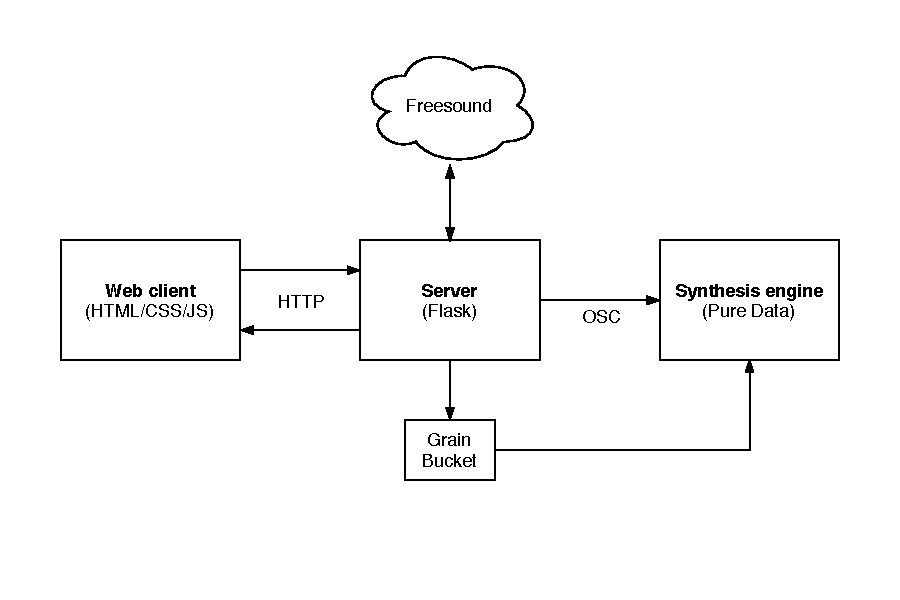
\includegraphics[width=\linewidth]{../img/granabular-system.pdf}
	\caption{System block diagram.}
	\centering
\end{figure}

\subsection{Synthesis engine}

Tes

\subsection{Web server}

\subsection{Web client}

\section{Future work}

\section{Conclusions}


%ACKNOWLEDGMENTS are optional
%\section{Acknowledgments}

% The following two commands are all you need in the
% initial runs of your .tex file to
% produce the bibliography for the citations in your paper.
\bibliographystyle{abbrv}
\bibliography{nime-references}  % sigproc.bib is the name of the Bibliography in this case
% You must have a proper ".bib" file
%  and remember to run:
% latex bibtex latex latex
% to resolve all references
%
% ACM needs 'a single self-contained file'!
%

\end{document}
